In this chapter, we evaluate the instrumentation for checking memory safety.
We employed the instrumentation in \symbiotic and ran it on benchmarks from SV-COMP 2018.

We used all the benchmarks from the official \emph{MemSafety} category along
with the benchmarks from the subcategory \emph{TerminCrafted} which was not
included in the official SV-COMP 2018. The benchmarks from these categories are
programs in C and they can contain either no violation of memory safety, or the
following errors:
\begin{itemize}
  \item invalid memory deallocation, e.g. double free error,
  \item invalid pointer dereference,
  \item memory leaks.
\end{itemize}
There were 390 benchmarks in total, 140 of them containing some
memory safety violation, 250 of them safe.

\symbiotic answers \emph{true} if no error location is reachable. If some error
location is reachable, it answeres \emph{false} and gives information about a
type of the error (e.g.  invalid dereference or memory leak). If \symbiotic
cannot decide the reachability, it answers \emph{unknown}. If it runs out of
time, i.e.~the given time limit was exceeded, the answer is \emph{timeout}. All
\emph{true} and \emph{false} answers \symbiotic gave were correct.


\section{Comparison of Configurations}
In this section, we compare three configurations introduced in
Chapter~\ref{chap:memsafety}: the basic approach (one-phase instrumentation
without any plugins, denoted as \emph{basic}), the enhancement with a pointer
analysis as a plugin (denoted as \emph{ePTA}) and the staged instrumentation
with the constant-time checks (denoted as \emph{staged}).

We ran \symbiotic with these configurations on the above mentioned benchmarks
with the CPU time limit set to 120~s. All the following measurements were taken
on machines with \textit{Intel(R)~Core(TM)~i7-3770} CPU that run on 3.40GHz
frequency and dispose of 8~GB of memory. The memory limit was set to 8~GB. We
used the utility \emph{Benchexec}~\cite{Beyer2015} for reliable measurement of
consumed resources.

\begin{table}[t]
\begin{tabular}{V{2} p{6cm} | C{1.5cm}|  C{1.5cm} | C{1.5cm} V{2}}
 \Xhline{2\arrayrulewidth}
 & \textbf{basic} & \textbf{ePTA} & \textbf{staged} \\
 \Xhline{2\arrayrulewidth}
 size before instrumentation & 155801 & 155801 & 155801 \\
 \hline
 size after instrumentation  & 322058 & 192496 & 171348 \\
 \hline
 inserted calls (total)    & 166257 & 36695 & 15547 \\
 \hline
 inserted calls (average)  & 426 & 94 & 39 \\
 \Xhline{2\arrayrulewidth}
\end{tabular}
\caption{The comparison of the three configurations for the memory safety
instrumentation. Size is given by the number of instructions of a program.}
\label{tab:numbers}

\end{table}

As for the number of inserted instructions, we present the experimental results
in Table~\ref{tab:numbers}. The first two rows of the table show the total size of
the benchmarks expressed with the number of LLVM instructions before and after
instrumentation for each configuration. The other two rows show the cumulative and
average number of inserted \texttt{call} instructions. Note that the
total size before instrumentation is 155801 instructions, which is 400
instructions on average. This means that with the basic approach, the final code
after instrumentation is of more than double size. Evidently, the number of
inserted instructions significantly decreases with each enhancement. This is
also depicted in Figure~\ref{fig:box} that shows the box plot for each
configuration.

\begin{figure}[h]
  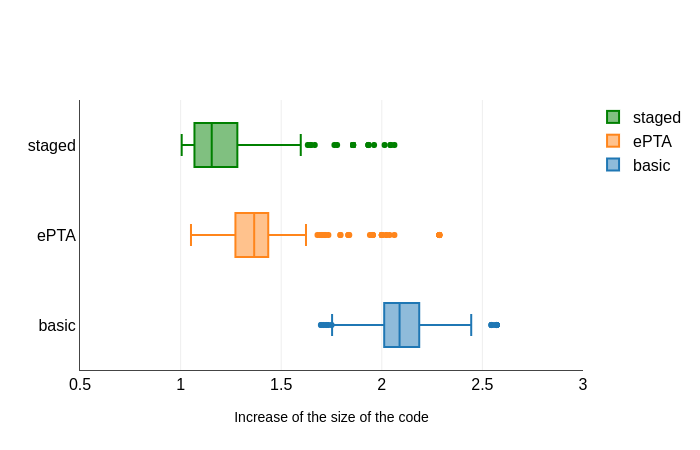
\includegraphics[width=\textwidth]{charts/box.png}
  \caption{The box plots for each of the three configurations for the memory safety instrumentation. The $x$-axis describes the ratio of the number of instructions after instrumentation to the number of instructions before instrumentation.}
  \label{fig:box}
\end{figure}

The reduced number of inserted instructions had indeed a positive effect on the
answers of \symbiotic as shown in Table~\ref{tab:answers}. When using the basic
approach, \symbiotic did not manage to decide 139 benchmarks in the given time
limit. With a pointer analysis, the number of timeouts slightly decreased. The
most significant improvement was achieved with the staged instrumentation:
\symbiotic ran out of time only in 71 cases. The both enhancements had impact
especially on the benchmarks that did not contain any violation of memory
safety. Observe that \symbiotic was able to reveal the memory violations in
almost all benchmarks that were labeled as unsafe in the given time limit with
all the configurations of instrumentation.

\begin{table}[t]
\begin{tabular}{V{2} c |  c |  c |  c V{2}}
 \Xhline{2\arrayrulewidth}
 & \textbf{basic} & \textbf{ePTA} & \textbf{staged} \\
 \Xhline{2\arrayrulewidth}
 true     & 116 & 123  & 183 \\
 \hline
 false    & 132 & 133  & 135 \\
 \hline
 timeout  & 139 & 130  & 71 \\
 \Xhline{2\arrayrulewidth}
\end{tabular}
\caption{The numbers of \emph{true}, \emph{false} and \emph{timeout} answers
given by \symbiotic when using the three configurations for the memory safety
instrumentation.}
\label{tab:answers}

\end{table}

We also measured the CPU running times of the instrumentation process. The
instrumentation using the basic approach took approximately 40~ms on average.
Even though the enhanced configurations of the instrumentation need to
additionally perform a pointer analysis at the beginning, the running times increased
insignificantly as showed in Figure~\ref{fig:times_chart}.

\begin{figure}[h]
  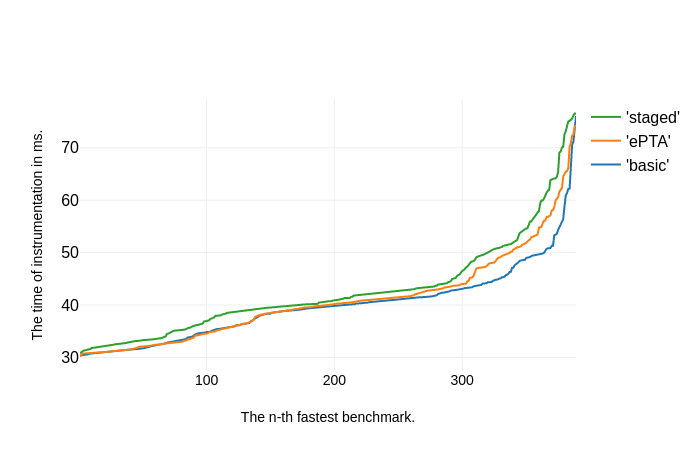
\includegraphics[width=\textwidth]{charts/instr_times_chart.png}
  \caption{The CPU running times of instrumentation when using
  the three configurations for the memory safety instrumentation.}
  \label{fig:times_chart}
\end{figure}

\section{SV-COMP 2018}

\symbiotic proved its abilities in SV-COMP~2018, where it won the first place
in the official \emph{MemSafety} category. There were 326 benchmarks in
total\footnote{\url{https://sv-comp.sosy-lab.org/2018/benchmarks.php}}.

In Table~\ref{tab:results} we present the results of \symbiotic,
\textsc{PredatorHP}~\cite{predatorhp} which was placed second, and \textsc{UKojak}~\cite{ukojak} which was
third. The results were published at the official website of
SV-COMP~2018\footnote{\url{https://sv-comp.sosy-lab.org/2018/results/results-verified/}}.
None of the tools reported any incorrect answer.


Table~\ref{tab:score} shows that not only \symbiotic scored the most points,
but it was also the fastest. \symbiotic managed to solve the benchmarks almost
seven times faster than \textsc{PredatorHP} and thirty-five times faster that
\textsc{UKojak}. This achievement is also visible in the quantile plot in
Figure~\ref{fig:quantile}. The difference

\begin{table}[!t]
\begin{center}\setlength{\tabcolsep}{5pt}
\begin{tabular}{V{2} c| c|c|c|c|c|c|c V{2}}
\toprule[1pt]
 & & \multicolumn{2}{c}{\bf \symbiotic}
& \multicolumn{2}{|c|}{\bf \textsc{PredatorHP}}
& \multicolumn{2}{c V{2}}{\bf \textsc{UKojak}}\\
\midrule[1pt]
\mr{category} &\scriptsize number of
& \mr{solved} &\scriptsize safe
& \mr{solved} &\scriptsize safe
& \mr{solved} &\scriptsize safe\\
%\cmidrule(lr{.75em}){4-4} \cmidrule(lr{.75em}){6-6} \cmidrule(lr{.75em}){8-8}
\cline{4-4} \cline{6-6} \cline{8-8}
& \scriptsize benchmarks
&&\scriptsize unsafe &&\scriptsize unsafe &&\scriptsize unsafe\\
\midrule[1pt]
% --------------------------------------------------------------------------------------
\mr{Arrays} & \mr{69}      & \mb{62}  &\scriptsize 44 & \mr{7} &\scriptsize 0 & \mr{44}  &\scriptsize 27 \\
\cline{4-4}\cline{6-6}\cline{8-8}
           &               &        &\scriptsize 18 &          &\scriptsize 7 &           &\scriptsize 17 \\
\midrule
\mr{Heap} & \mr{180}    & \mr{145} &\scriptsize 55 & \mb{148} &\scriptsize 66 & \mr{51} &\scriptsize 26 \\
\cline{4-4}\cline{6-6}\cline{8-8}
          &                &       &\scriptsize 90 &          &\scriptsize 82 &         &\scriptsize 25\\
\midrule
\mr{LinkedLists} & \mr{51} & \mr{27} &\scriptsize 3 & \mb{43} &\scriptsize 19 & \mr{4}  &\scriptsize 0 \\
\cline{4-4}\cline{6-6}\cline{8-8}
          &      &                 &\scriptsize 24 &          &\scriptsize 24 &          &\scriptsize 4\\
\midrule
\mr{Other} & \mr{26}       & \mb{26} &\scriptsize 23& \mr{18} &\scriptsize 16 & \mr{23} &\scriptsize 23 \\
\cline{4-4}\cline{6-6}\cline{8-8}
          &      &                  &\scriptsize 3 &          &\scriptsize 2 &         &\scriptsize 0 \\
\midrule[1pt]

\midrule[1pt]
\mr{total} & \mr{326} & \mb{260} &\scriptsize 125 & \mr{216} &\scriptsize 101 & \mr{122} &\scriptsize 76  \\
\cline{4-4}\cline{6-6}\cline{8-8}
           &          &          &\scriptsize 135 &          &\scriptsize 115 &         &\scriptsize 46\\
\bottomrule[1pt]
\end{tabular}
\vspace*{1em}
\caption{Numbers of solved benchmarks by each of the three winner of SV-COMP~2018.}
\label{tab:results}
\end{center}
\end{table}


\begin{table}[t]
\centering
\begin{tabular}{V{2} c|c|c|c V{2}}
\Xhline{2\arrayrulewidth}
          & \textbf{\symbiotic} & \textbf{\textsc{PredatorHP}} & \textbf{\textsc{UKojak}} \\
\hline
score     & 411        & 286                   & 265               \\
\hline
CPU times & 310 s      & 2100 s                & 11 000 s\\
\Xhline{2\arrayrulewidth}
\end{tabular}
\caption{Score and CPU times (without timeouts) of the three winners of SV-COMP~2018.}
\label{tab:score}

\end{table}

\begin{figure}[h]
  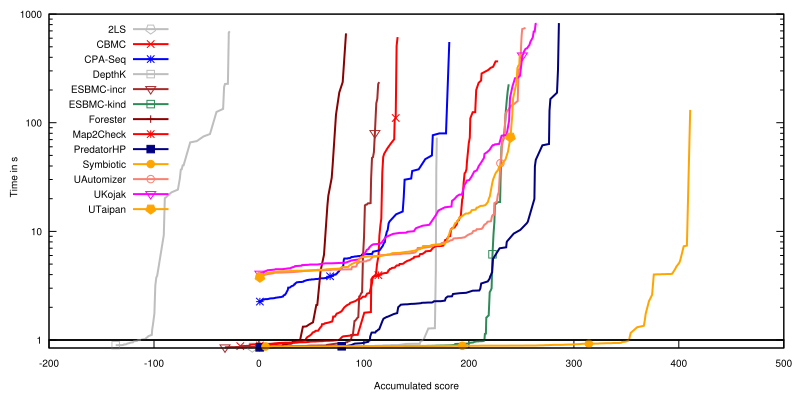
\includegraphics[width=\textwidth]{charts/quantilePlot-MemSafety.png}
  \caption{The quantile plot for the category \emph{MemSafety} taken from
  \url{https://sv-comp.sosy-lab.org/2018/results/results-verified/quantilePlot-MemSafety.svg}}
  \label{fig:quantile}
\end{figure}
